\section{Problema 2}

\subsection{Enunciado}
El enunciado nos plantea una situación en donde tenemos $n$ localidades conectadas entre si, mediante uno o más enlaces telefónicos. La empresa desea que la conectividad entre todas las ciudades nunca se pierda, por lo que está interesada en invertir en cableado subterraneo indestructible. El precio de conectar las distintas localidades varía según las mismas, por lo que la empresa nos pide que hallemos la forma de conectar todas las ciudades y que ninguna quede incomunicada, de forma de que la inversión en éste nuevo cableado subterraneo sea mínima.

\subsection{Soluci\'on}
Al presentarnos éste problema, inmediatamente pensamos que era posible reprentarlo mediante un problema de grafos. El mismo representaría todo la red de conectividad de la empresa telefónica, los vértices del mismo representarían las localidades y las aristas entre los distintos nodos representarían el costo del cableado subterraneo entre las ciudades que uniera la misma.
Dicho ésto, el problema se reducía, entonces, a hallar un grafo cuyas aristas permitan ir de una ciudad a cualquier otra del grafo, y además, a que esas aristas tengan un costo mínimo de construcción. En otras palabras, necesitamos un algoritmo que nos calcule, dado un grafo cualquiera, el arbol generador mínimo (AGM). El agm es un grafo que contiene los mismo vértices que el original, pero sólo contiene v-2 aristas (siendo v la cantidad de vértices), que unen todo el grafo y cuyo peso total es mínimo.
Para el problema, hemos implementado una clase propia de Grafo, representanda por una lista de adyacencia, y utilizado el conocido y demostrado Algoritmo de Prim para generar el AGM. El mismo consiste en, dado un grafo cualquiera, agarrar un vértice del mismo al azar, y agregarlo al AGM (que originalmente no tenía ningún vértice ni aristas). Luego, agregamos al grafo la arista de menor peso que conecte al vértice recién insertado con un vértice que no esté en el agm. Para ello, agregamos todas las aristas del vértice en una cola de prioridad, y vamos desencolando hasta que encontremos una arista que tenga un extremo en el agm y otro no (es decir, tengo un sólo vértice en el árbol). Una vez que encontramos dicha arista, agregamos el vértice que no estaba al AGM y también la arista. El proceso debe ser repetido, de la misma forma, con todos los vértices del grafo, es decir, hasta que la cantidad de vértices que hay en el árbol sea la misma que había en el grafo original. Ésta es la forma en que se describe el algoritmo de prim y la forma en que actúa nuestro algoritmo, por lo que podemos decir que la implementación realizada se corresponde con dicho algorítmo.

\subsection{Pseudoc\'odigo}
En código del ejercicio básicamente hace una cosa: lee el archivo de entrada, y procesa las lineas y va creando las distintas instancias del ejercicio. La lógica del problema está toda delegada en la clase Grafo, que es la que se encarga de modelar las localidades y sus enlaces (el grafo en sí), y luego, una vez modelado, de crear el propio AGM. El agm está implementado a partir del algoritmo de prim, que busca para cada vertice nuevo agregado, la arista de menor peso que lo conecte con un vertice que no esté en el grafo y la agrega.
La lógica del ejercicio podría dividirse, de acuerdo a lo recién mencionado, de la siguiente manera:

\begin{codebox}
\Procname{$\proc{CrearGRafo}$ (\textbf{String} $instancia$)}{g}{Grafo}
\li	Grafo g;
\li	para cada enlace de la instancia: \Do
\li		agrego el vertice 1
\li		agrego el vertice 2
\li		agrego la arista entre v1 y v2
\End
\li	devuelvo el grafo 
\end{codebox}

\begin{codebox}
\Procname{$\proc{getAgm}$()}{g}{Grafo}
\li	Grafo agm;
\li	agrego un vertice al azar del grafo al agm
\li	marco el vertice agregado como visitado
\li	agrego las aristas del vertice visitado a la cola de prioridad
\li	para cada vertice en grafo: \Do
\li		obtengo la arista de menor peso de la cola
\li		miro los dos vertices de la arista
\li		si alguno no fue visitado:\Do
\li			agrego la arista minima al agm
\li			marco el vertice como visitado
\li			agrego las aristas del vertice a la cola de prioridad
\End
\End			
\li	devuelvo el agm
\end{codebox}

\subsection{Analisís de complejidad}	
En éste ejercicio, para el análisis de la complejidad utilizaremos la información conocida de la documentación de Java, ya que en su gran mayoría, la complejidad de ejercicio depende de las estructuras que utilizamos para resolver el mismo.
Para el análisis, sólo vamos a tener en cuenta lo que nos cuesta resolver el ejercicio, y no la forma en que leemos los archivos de entrada. Por ello, asumimos que leer de la entrada no afecta a la complejidad del algoritmo. Por su parte, y una vez que ya tenemos la entrada cargada en memoria, recrear las instancias va a depender de la cantidad de vértices que tengamos, y de las aristas que tenga cada vértice. Ingresar un vértice es $O(1)$ para cada uno de ellos, lo mismo que ingresar las n aristas que tenga dicho vértice. Por lo tanto, la complejidad de recrearlo será de $O(v + c) = O(v)$, siendo v la cantidad de vértices del grafo y c una constante, dependiente de las aristas que tenga cada vértice (el cual podemos obviar).
Luego, para la resolucion del problema, recorremos 1 vez cada vértice, que tenemos almacenado en un arrayList. Obtener cada vértice es $O(1)$, por lo que recorrer los n vértices tendrá un costo de $O(n)$. 
Luego, para cada vértice, agregamos las aristas que lo tienen como uno de los extremos a una cola de prioridad. En el peor de los casos (por ejemplo, para el último vértice, donde ya ingresamos todas las aristas de todos los vértices), vamos a tener que ingresar e aristas (donde e es al número total de aristas del grafo). En ese caso, las acciones básicas de la cola de prioridad (ingresar un elemento, o quitar el primer elemento), tienen un costo de $O(\log e)$, por lo que realizarlo para todos los vértices, el costo total de las operaciones de la cola sería de $O(v \log e)$.
Por útlimo, quedan operaciones básicas, como comparar valores, ver si el vértice está visitado o agregar el vértice al agm, que en todos los casos, son $O(1)$.
Finalmente, la complejidad de nuestra solución será de \[O(v) + O(v) + O(v \log e) = O(v + v \log e)\] cumpliendo de ésta forma lo pedido en el enunciado, que establecía que el ejercicio debía resolverse en, como mucho, $O(m*v)$.
\subsection{Tests y Gráficos}
Con respecto a los tests realizados, los mismos no se hicieron en cuanto a la complejidad (ya que al utilizar estructuras primitivas de java, podemos asegurar que la complejidad de cada una de sus operaciones es la que aparece en la documentación de ellas y por tanto, es la que detallamos en el apartado anterior), sino en cuanto a la cantidad de ciclos que realiza cada solución (más precisamente, la creación del árbol generador mínimo) para distintas instancias, de acuerdo a la cantidad de vértices (localidades) y aristas (enlaces) que posee cada una.
Como podemos apreciar en los siguientes gráficos, la cantidad de ciclos, para grafos en donde la cantidad de aristas es la misma, es proporcional a la cantidad de aristas totales que haya en el vértices, sin importar cuántos vértices haya o cuántas aristas por vértice tenga el grafo.
Para mostrar ésto, realizamos dos gráficos, luego de correr varias pruebas de las siguientes instancias: por un lado, utilizamos como variable la cantidad de vértices, manteniendo las aristas por vértices constantes (figura 1). Y por otro lado, hemos variado la cantidad de vértics, manteniendo constantes la cantidad de aristas por vértice (figura 2). En ambos casos, la cantidad TOTAL de aristas del grafo se mantenía igual.
Como podemos apreciar en primer gráfico, dónde hemos mantenido la cantidad de aristas por vértice constante, vemos que el comportamiento es el de esperar: a mayor cantidad de vértices, mayor cantidad de ciclos.  En el mismo hemos corrido instancias con 10, 20, 30 y 40 aristas y hecho un promedio de los ciclos en 10 ejecuciones y, en su mayoría, se ha mantenido éste criterio. Es de esperar que, como pasa en el caso con más aristas, no siempre se cumpla que la cantidad de ciclos crece ya que, al tener que analizar muchas aristas, es posible que encuentre una arista de mayor peso en el primer paso, o bien en el último, siendo que los pesos de las aristas son creados de forma aleatoria.
\begin {center}
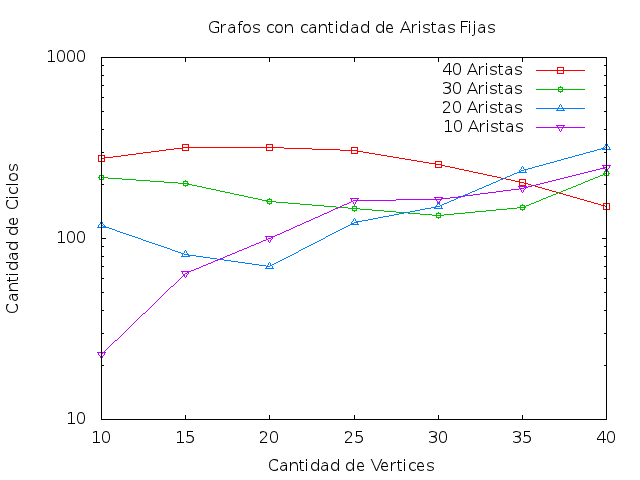
\includegraphics[width=8cm]{./graficos/graficos_aristas_fijas.png}
% grafico.eps: 0x0 pixel, 300dpi, 0.00x0.00 cm, bb=50 50 410 302
\end {center} 
Por otro lado, podemos apreciar el gráfico que hemos creado a partir de las instancias que poseen vértices fijos. Como vemos, es muy parecido al gráfico anterior, como era de esperar según nuestras suposiciones. Nuevamente, en el caso de mayor cantidad de vértices fijos, no siempre se cumple que a más aristas, más cantidad de ciclos, por la misma razón que en gráfico anterior. Pero, en promedio, podemos decir que a mayor cantidad de aristas totales en el grafo, más cantidad de ciclos, sin importar cómo estén distribuidas éstas: ya sea teniendo más aristas por vértice, o bien teniendo más vértices.
\begin {center}
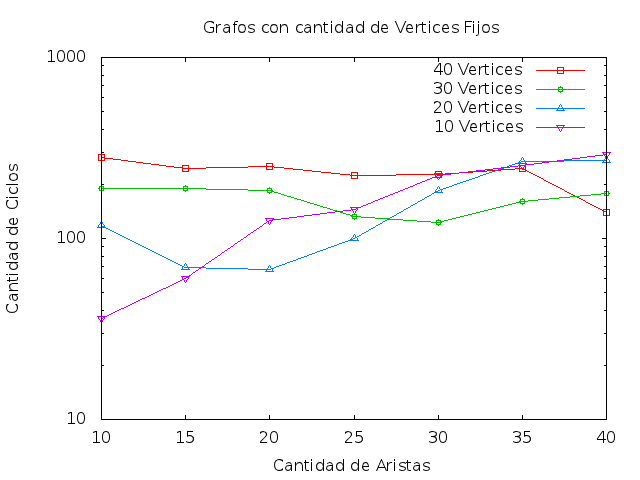
\includegraphics[width=8cm]{./graficos/graficos_vertices_fijos.png}
% grafico.eps: 0x0 pixel, 300dpi, 0.00x0.00 cm, bb=50 50 410 302
\end {center} 


\subsection{Conclusiones}
A partir del problema dado, hemos podido modelar a partir de la teoría de grafos. De ésta forma, e interpretando qué es lo que nos pide el enunciado, hemos podido resolver el problema a partir de un algoritmo que es conocido y, de esa forma, podemos afirmar que estamos dando la solución correcta. 
En ésta caso, modelamos nuestras localidades y los distintos precios que costaban unirlas a partir de un grafo conexo, no dirigido. Para éstos grafos, es posible hallar un grafo de peso mínimo que conecte todas las ciudades, conocido también como árbol generador mínimo (agm). Precisamente, ésto es lo que nos pedía el enunciado: hallar la forma de conectar todas las ciudades de forma tal que el coste de unirlas todas sea mínimo. Con nuestro planteo, logramos responder dicho problema, teniendo en cuenta, además, la complejidad pedida para resolverlo. La misma fue lograda no sólo implementando un algoritmo conocido, como es el de prim, sino que se fue cuidadoso a la hora de elegir las estructuras de datos utilizadas para mantenernos dentro de la cota estipulada.
Por último, pudimos mostrar que nuestro algoritmo se comporta de manera similar para cuando la cantidad de aristas total del grafo es la misma, sin importar si éstas se consiguen agregando más vértices, o bien, agregando más aristas por vértices.
